
%%%%%%%%%%%%%%%%%%%%%%%%%%%%%%%%%%%%%%%%%%%%%%%%%%%%%%%%%%%%%%%%%%%%%%%%
%Para las ecuaciones siempre es Ec.(n).
%Para las figuras siempre es Fig.n, incluso en el caption de la figura. Tambien las Tablas
%Para las referencias es [n]
%%%%%%%%%%%%%%%%%%%%%%%%%%%%%%%%%%%%%%%%%%%%%%%%%%%%%%%%%%%%%%%%%%%%%%%%

\documentclass[
reprint,
%notitlepage,
%superscriptaddress,
%groupedaddress,
%unsortedaddress,
%runinaddress,
%frontmatterverbose, 
%preprint,
%showpacs,preprintnumbers,
%nofootinbib,
%nobibnotes,
%bibnotes,
%11 pt,
amsmath,
amssymb,
aps,
%pra,
%prb,
%rmp,
%tightenlines %esto hizo el milagro de sacar los espacios en blancos estocásticos (?)
 %prstab,
%prstper,
%floatfix,\textbf{}
]{revtex4-1} %Instalar primero para usarlo. Paquete malo.

%\documentclass[onecolumn, aps, amsmath,amssymb ]{article}
\usepackage{lipsum}  
\usepackage{graphicx}% Include figure files
\usepackage{subfig}
\usepackage{braket}
\usepackage{comment} %comment large chunks of text
\usepackage{dcolumn}% Align table columns on decimal point
\usepackage{bm}% bold math
%\usepackage{hyperref}% add hypertext capabilities
\usepackage[mathlines]{lineno}% Enable numbering of text and display math
%\linenumbers\relax % Commence numbering lines
\usepackage{mathtools} %% Para el supraíndice

\usepackage[nice]{nicefrac}

%%%%%%%El Señor Español%%%%%%%%%%%%%%%%%%%%%%%%%%%
\usepackage[utf8]{inputenc} %acento
\usepackage[
spanish, %El lenguaje.
es-tabla, %La tabla y no cuadro.
activeacute, %El acento.
es-nodecimaldot %Punto y no coma con separador de números
]{babel}
\usepackage{microtype} %para hacerlo más bonito :33 como vos (?) 
%%%%%%%%%%%%%%%%%%%%%%%%%%%%%%%%%%%%%%%%%%%%%%%%%%%
%%%%%%%%% Para que las imágenes se queden dónde las quiero (?
\usepackage{float}
%%%%%%%%%%

%%%%%%%%Cambia a Fig de Figure%%%%%%%%%%
\makeatletter
\renewcommand{\fnum@figure}{Fig. \thefigure} 
\makeatother
%%%%%%%%%%%%%%%%%%%%%%%%%%%%%%%%%%%%%%%%
\raggedbottom


\begin{document}
%%%%%%%%%%%%%%%%%%%%%%%%%%%%%%%%%%Título%%%%%%%%%%%%%%%%%%%%%%%%%%%%%%%%%%%%%%
%%%%%%%%%%%%%%%%%%%%%%%%%%%%%%%%%%%%%%%%%%%%%%%%%%%%%%%%%%%%%%%%%%%%%%%%%%%%%%

\title{Pesos de los hexágonos}
\author{Evelyn~G.~Coronel}

\affiliation{
Tesis de Maestría en Ciencias Físicas\\ Instituto Balseiro\\}

\date[]{\lowercase{\today}} %%lw para lw, [] sin date

%\begin{abstract}

%\end{abstract} 
\maketitle
%%%%%%%%%%%%%%%%%%%%%%%%%%%%%%%%%%%%%%%%%%%%%%%%%%%%%%%%%%%%%%%%%%%%%%%%%%%%%%%%%%%
% Podemos usar cualquiera de los dos comandos: \input o \include para incluir el texto



\section{Dudas sobre los pesos}

Los pesos de los hexágonos son importantes para el cálculo de anisotropías, porque las anisotropías son pequeñas y eliminar todo factor espúreo es importante.

¿Por qué me trabé tanto? Cuando uso sólo 24 bines, los números entre el paper del 2018 y los que obtengo con mi código son parecidos. En cambio cuando otro bineado, como 360 bines, con el mismo código, hay una diferencia entre lo que se obtiene en el paper mencionado y el mi tesis.

¿Por qué creo que está pasando esto? Si el código funciona para 24 bines, como se muestra en la Fig.\,\ref{fig:all_24}, y cuando sólo cambio la cantidad de bines, como en las Fig.\,\ref{fig:sid_360} y \ref{fig:anti_360}, se ve que sigue la misma tendencia pero no los mismos números. Yo lo que yo creo es que tiene que ver con la precisión del cálculo. Para calcular cada punto, se realiza una división entre dos números, i.e. 
\begin{equation}
	\Delta N = \frac{\text{Los hexágonos integrados en un bin}}{\text{Todos los hexágonos integrados para cada bin}}
\end{equation}


\begin{figure}[H]
	\centering
	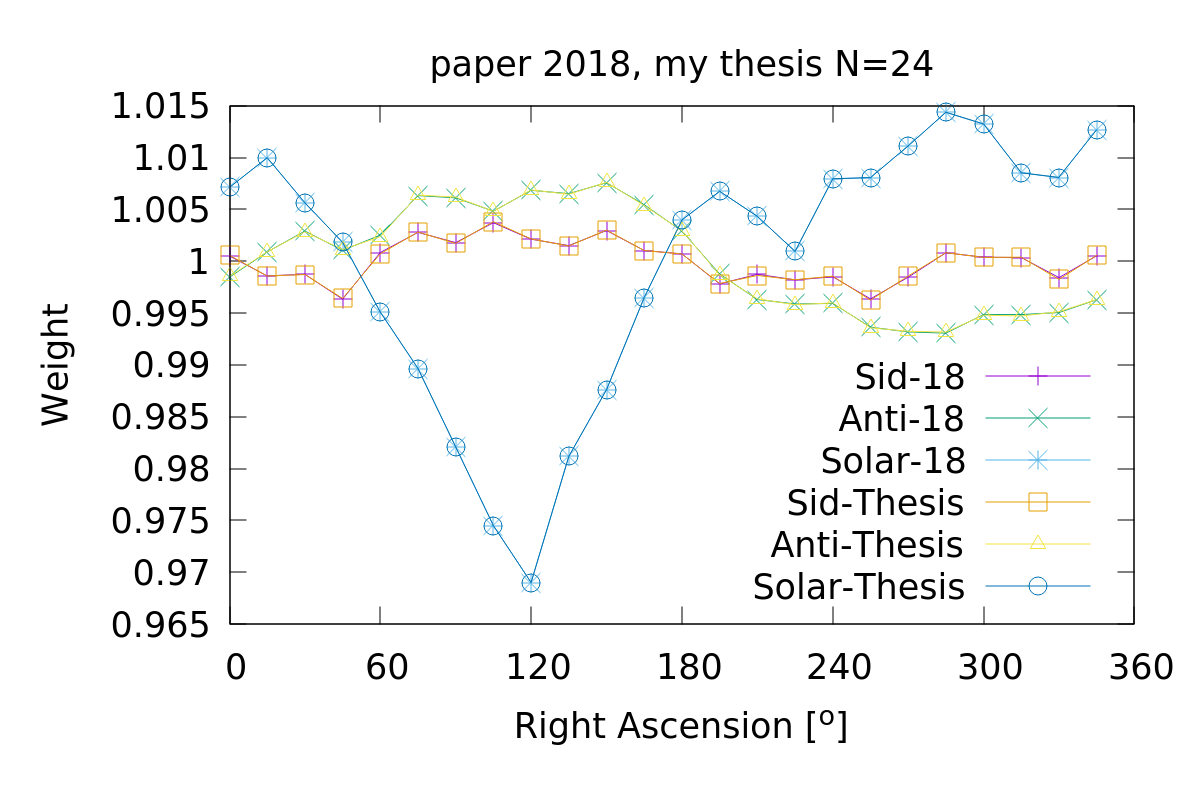
\includegraphics[width=0.45\textwidth]{Graficos/solar_anti_sid_my_and_paper_in_24.png}
	\caption{Usando 24 bines para las frecuencias sidérea, anti-sidérea y solar, se compara el paper del 2018 con lo que obtengo en la tesis.}
	\label{fig:all_24}
\end{figure}


En el caso de $N=24$, son dos números grandes, por lo tanto solo importan los primeros número a izquierda, pero para  $N=360$ es como menor. Durante la ejecución del programa, para cada valor de utc, se calcula a que bin corresponde esa entrada; verifiqué que el programa del paper y mío fuera iguales a cada paso, y constaté que no había diferencias.

Debido a esto, mi hipótesis es la diferencia entre ambos códigos es por la suma de hexágonos. Lo que me causa ruido de esto es que la diferencia entre los puntos del paper y de mi código, para la frecuencia sidérea,  no es ruido centrado en cero como esperaría que fuera si es un error en la precisión, como se muestra en la Fig.\ref{fig:error_360_sid}, lo que me hace dudar de mi hipótesis. En cambio para la frecuencia anti-sidérea, como se ve en la Fig.\ref{fig:error_360_anti}, el error no tiene ninguna modulación.

\begin{figure}[H]
	\centering
	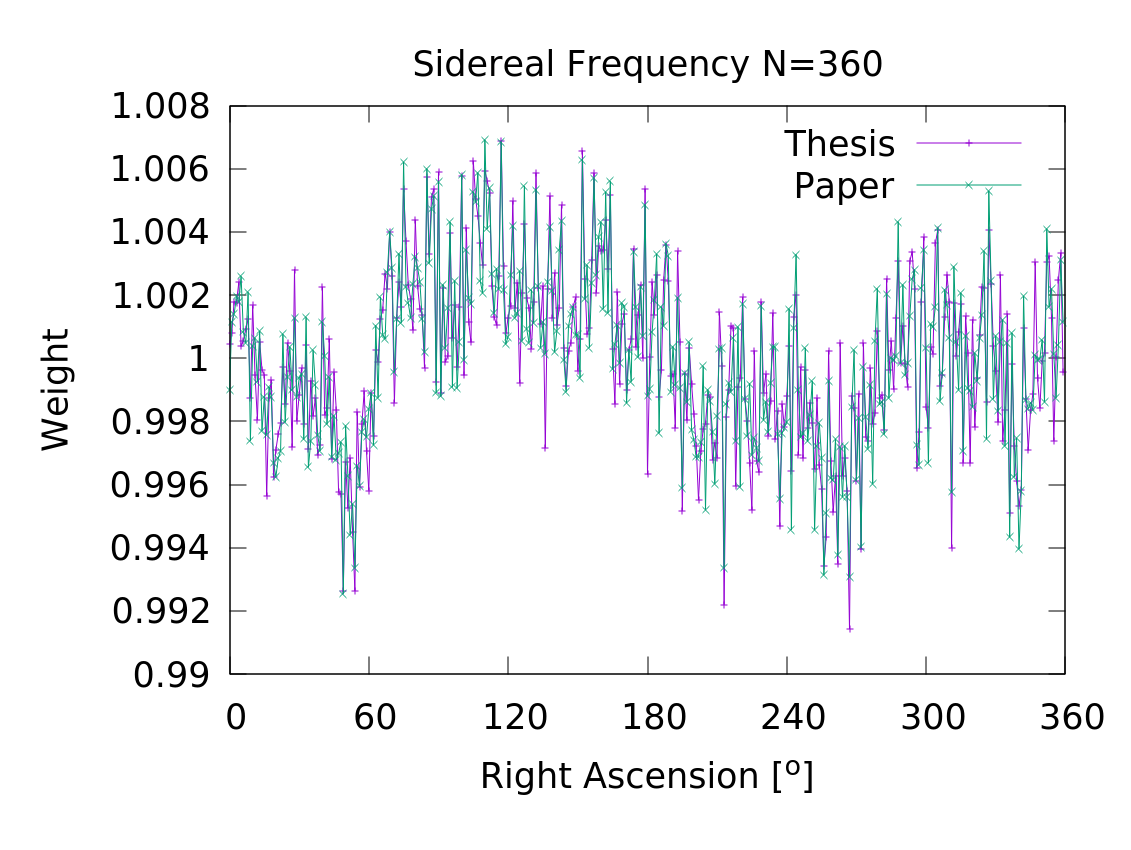
\includegraphics[width=0.45\textwidth]{Graficos/sidereal_my_and_paper_in_360.png}
	\caption{Usando 360 bines para la frecuencia sidérea.}
	\label{fig:sid_360}
\end{figure}


\begin{figure}[H]
	\centering
	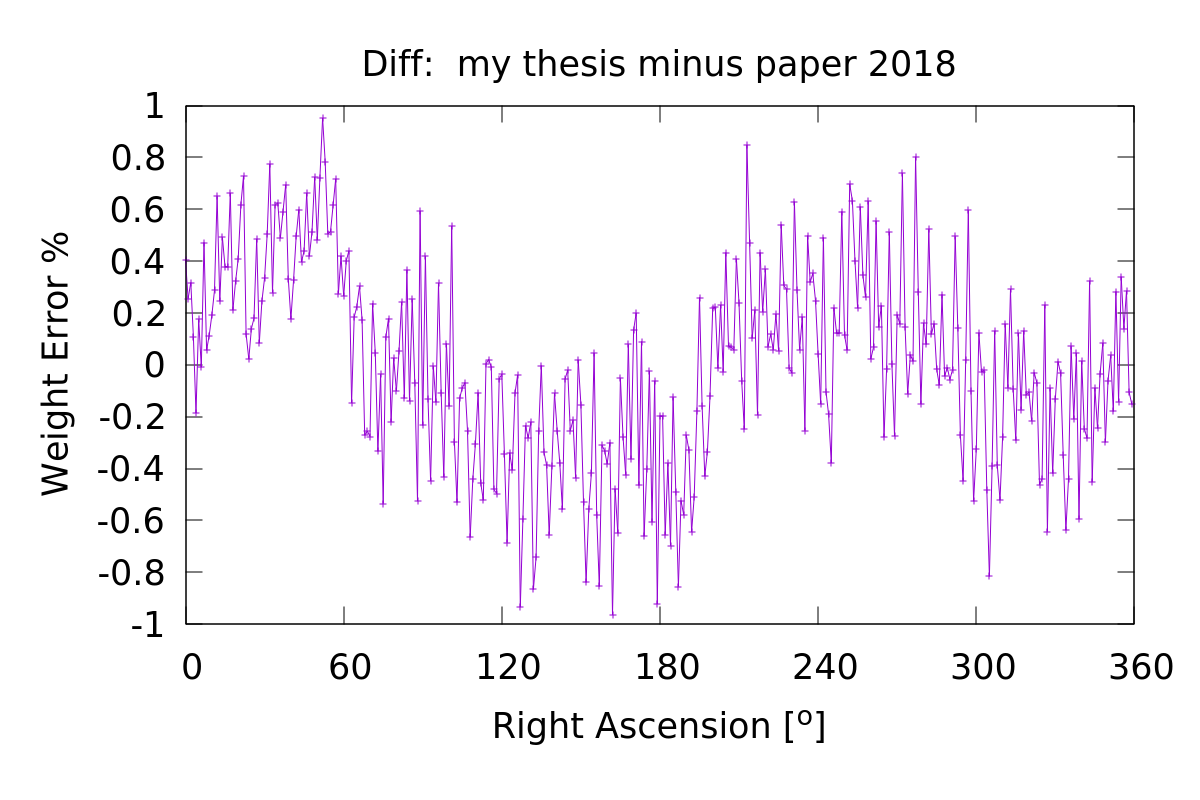
\includegraphics[width=0.45\textwidth]{Graficos/sidereal_my_and_paper_in_360_error.png}
	\caption{Usando los valores del paper como referencia, calculé el error porcentual con lo que yo obtengo para la frecuencia sidérea.}
	\label{fig:error_360_sid}
\end{figure}



\begin{figure}[H]
	\centering
	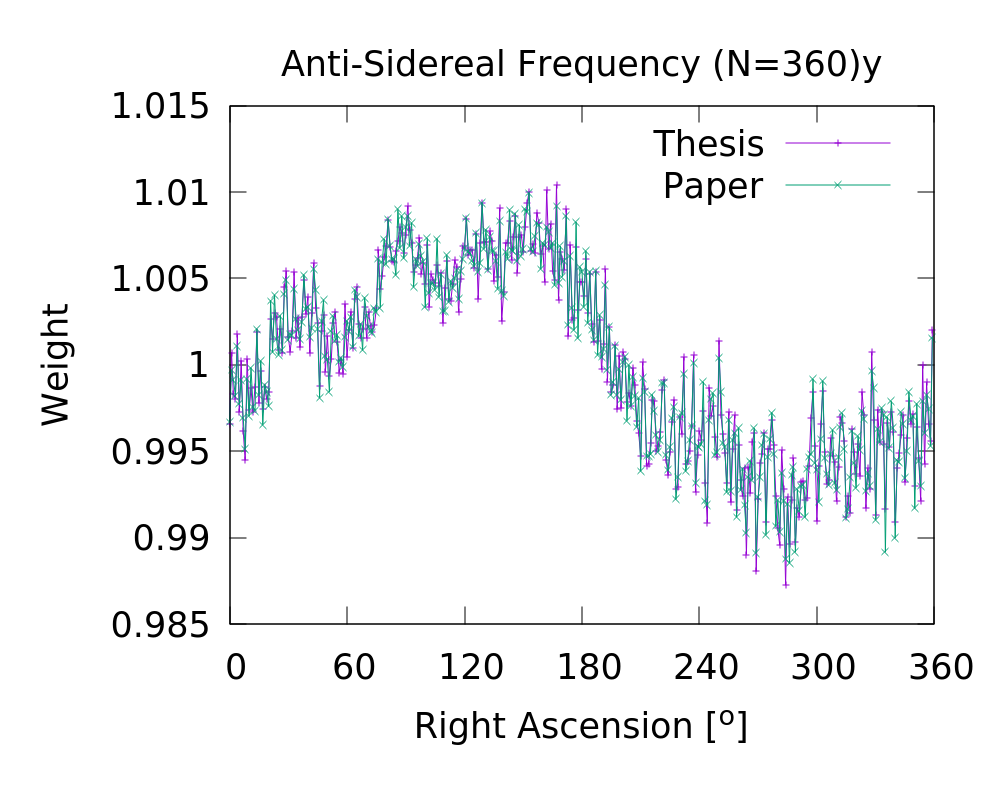
\includegraphics[width=0.45\textwidth]{Graficos/anti_my_and_paper_in_360.png}
	\caption{Usando 360 bines}
	\label{fig:anti_360}
\end{figure}


\begin{figure}[H]
	\centering
	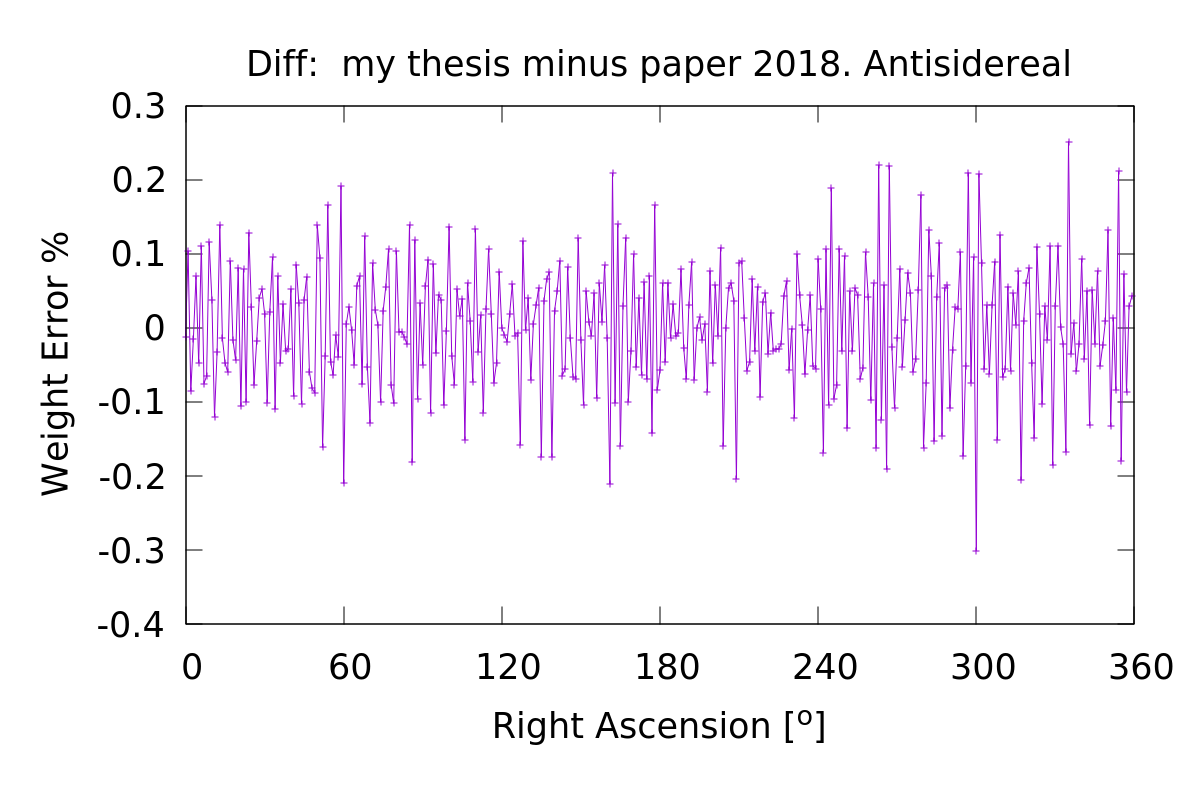
\includegraphics[width=0.45\textwidth]{Graficos/anti_my_and_paper_in_360_error.png}
	\caption{Usando los valores del paper como referencia, calculé el error porcentual de la frecuencia anti-sidérea.}
	\label{fig:error_360_anti}
\end{figure}



\section{Duda sobre los algoritmos}

Contexto: Yo quiero hacer el análisis de los pesos de los hexágonos para distintas frecuencias, por lo que esperaría que para cada frecuencia a analizar se utilice el mismo algoritmo para todos.

Mi duda: En el código del paper 18, el algoritmo hace distinción entre la frecuencia sidérea y las demás. Comparando ambos algoritmos, como se muestra en la Fig.\,\ref{fig:alter_24}, se ve que ambos dan un resultado similar para los pesos de los hexágonos a menos de un desfase de $75^o$ o $5\,$hrs sidéreas. Los gráficos de esta figura se hicieron con el mismo data set.

\begin{figure}[H]
	\centering
	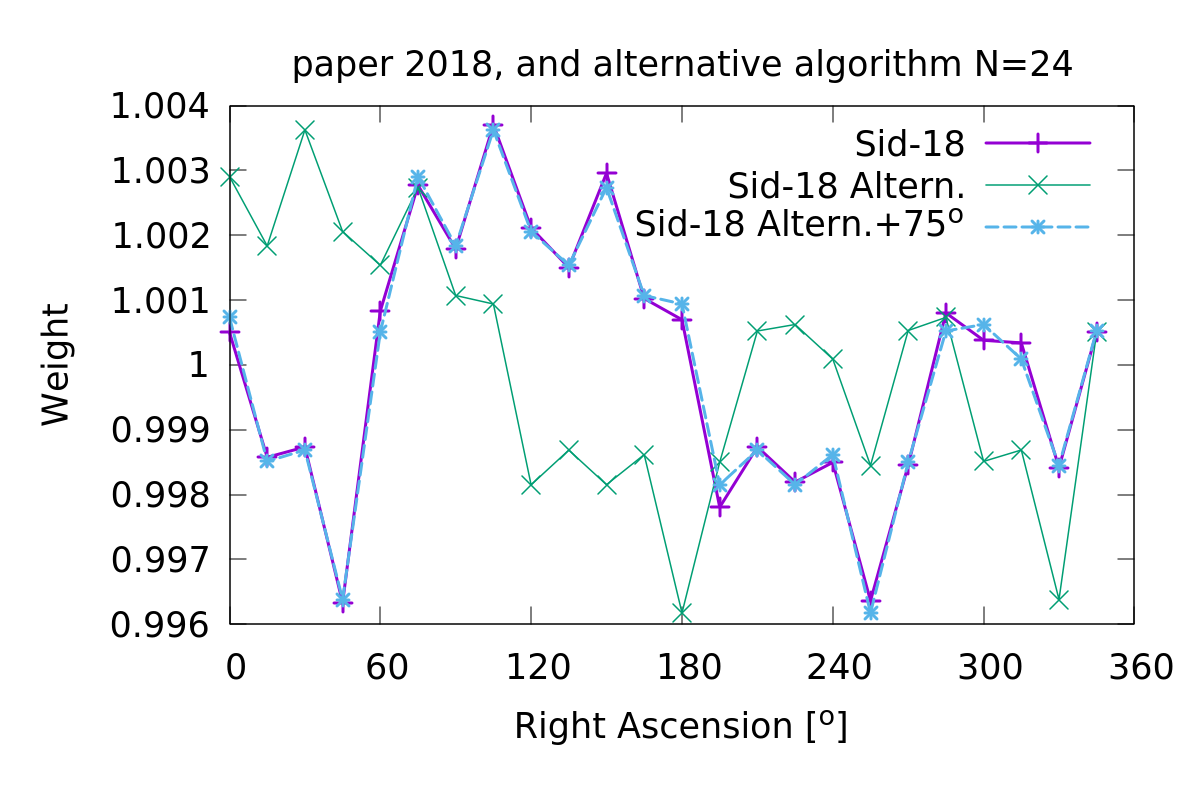
\includegraphics[width=0.45\textwidth]{Graficos/sidereal_paper_in_24_w_alter.png}
	\caption{Comparando el algoritmo alternativo con el utilizado en el paper 18 con resultados del mismo paper, para 24 bines.}
	\label{fig:alter_24}
\end{figure}


Otra cosa que me resultó curiosa fue que usando $N=360$, tengo problemas con la frecuencia solar, donde aparecen 0 cada 5 min, coincide con el rate de actualización del archivo de weather. Así usando este bineado, aparece ese problema, recomendaría no trabajar con bines de $1^o$ en ascensión recta.
\begin{figure}[H]
	\centering
	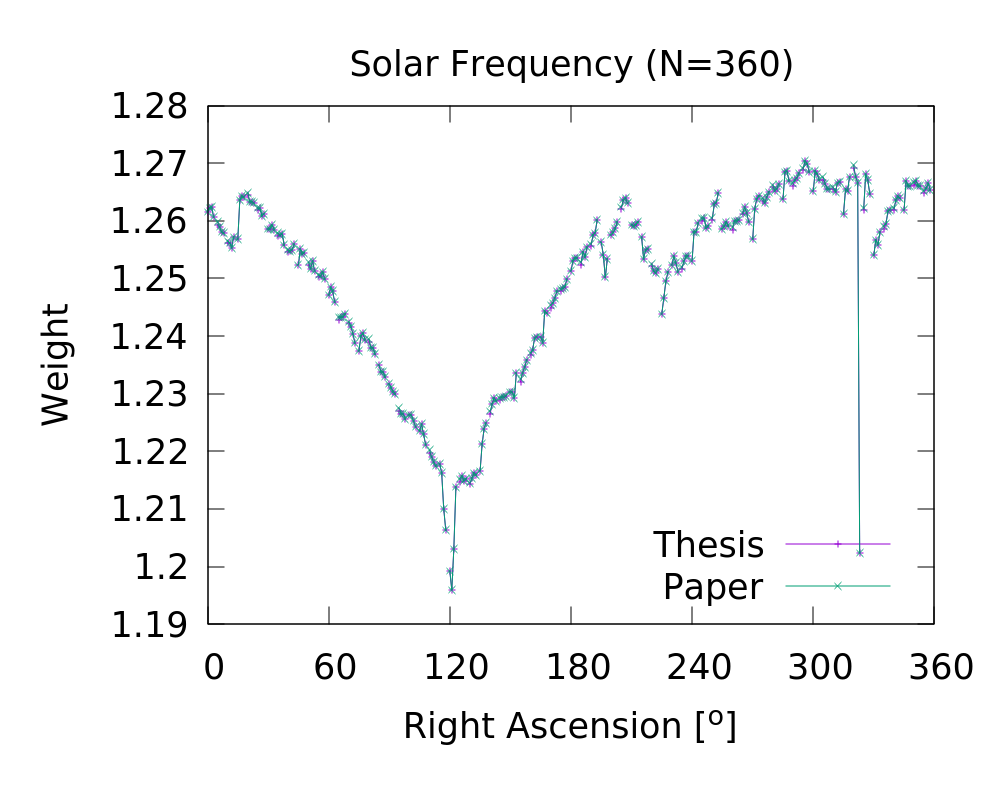
\includegraphics[width=0.45\textwidth]{Graficos/solar_my_and_paper_in_360_2.png}
	\caption{Usando 360 bines, nótese que la media es distinta a la figura anterior.}
	\label{fig:solar_360}
\end{figure}

\section{Para N=288}

El gráfico que me envió usted, sobre los pesos para estas frecuencias es la Fig.\,\ref{fig:all_288_paper}. La discusión sobre estos resultados en particular es análoga al caso para $N=360$, con la diferencia que no tengo valores de anómalos que se ven para la frecuencia solar, Fig.\,\ref{fig:solar_288}.
\begin{figure}[H]
	\centering
	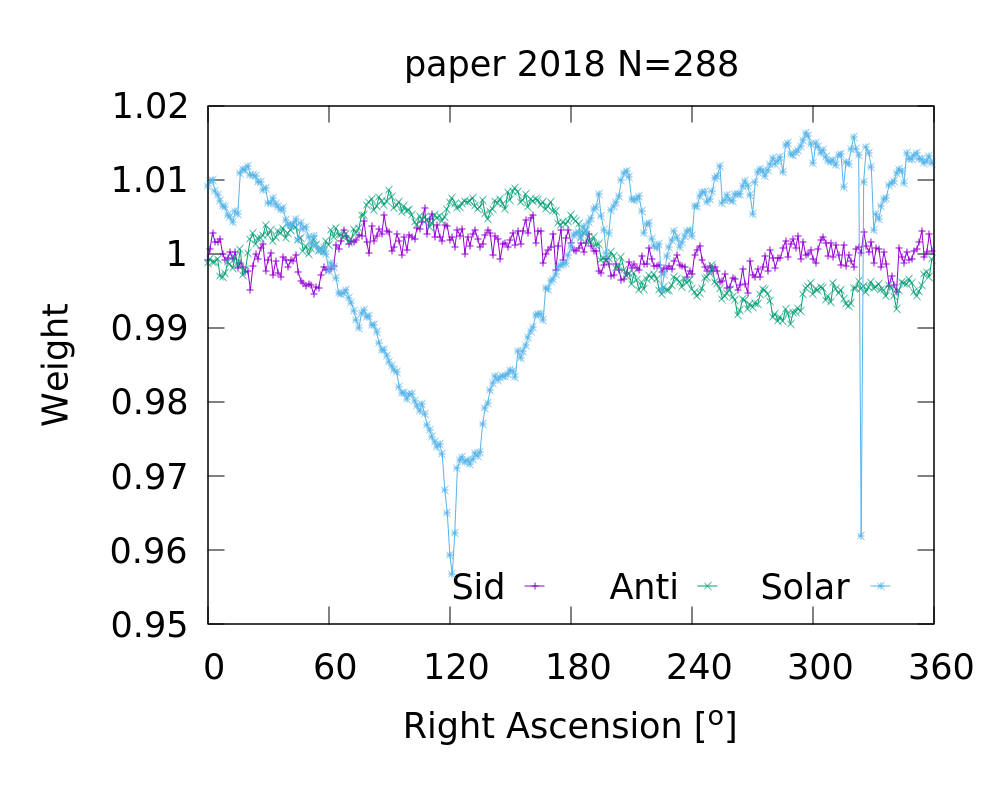
\includegraphics[width=0.45\textwidth]{Graficos/solar_anti_sid_paper2018_in_288.png}
	\caption{Los pesos para las tres frecuencias tal como se calcula en el paper del 2018.}
	\label{fig:all_288_paper}
\end{figure}



\begin{figure}[H]
	\centering
	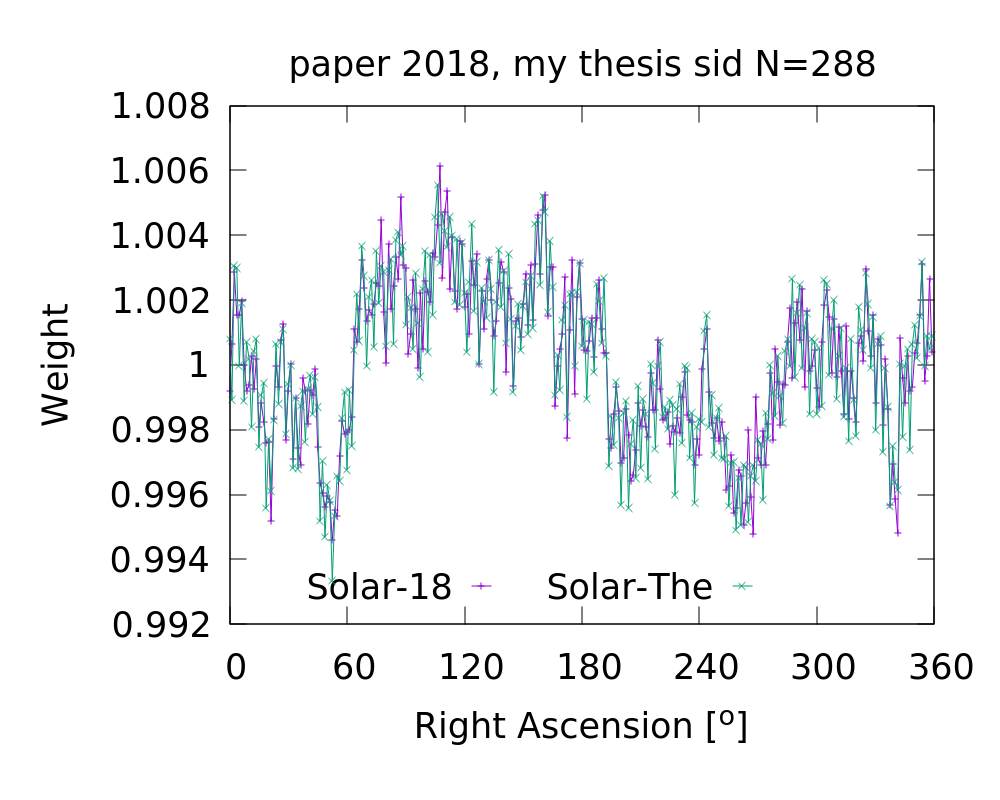
\includegraphics[width=0.45\textwidth]{Graficos/sidereal_my_and_paper_in_288.png}
	\caption{Comparando los resultados del paper con mi código para la frecuencia sidérea para N=288}
	\label{fig:sidereal_288}
\end{figure}


\begin{figure}[H]
	\centering
	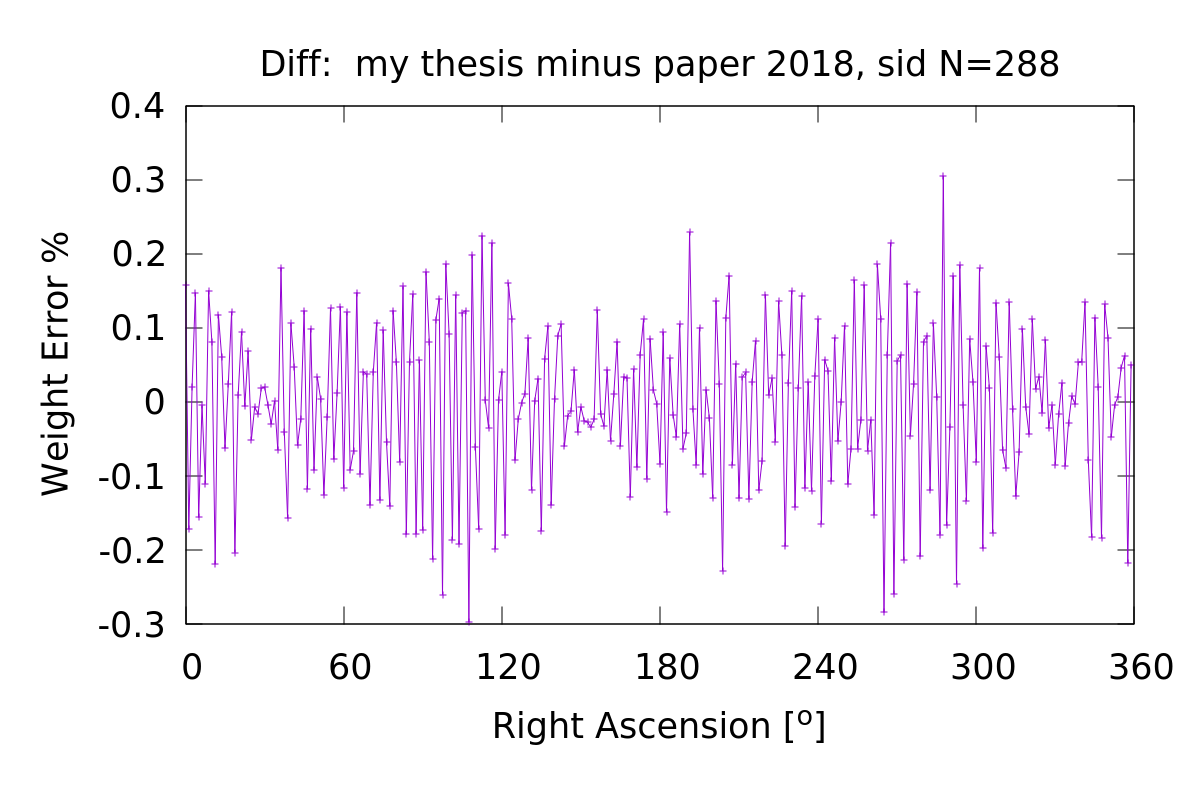
\includegraphics[width=0.45\textwidth]{Graficos/sidereal_my_and_paper_in_288_error.png}
	\caption{El error porcentual entre lo que obtengo en mi código, usando el paper de referencia.}
	\label{fig:error_288_sidereal}
\end{figure}


Ya en la Fig.\,\ref{fig:sidereal_288}, se ve que la media de los pesos es algo razonable comparándolo con N=360, Fig.\ref{fig:solar_360}. Además que el error porcentual, usando como referencia los resultados del paper del 2018, es pequeña. La misma se muestra en la Fig.\,\ref{fig:error_288_solar}.

\begin{figure}[H]
	\centering
	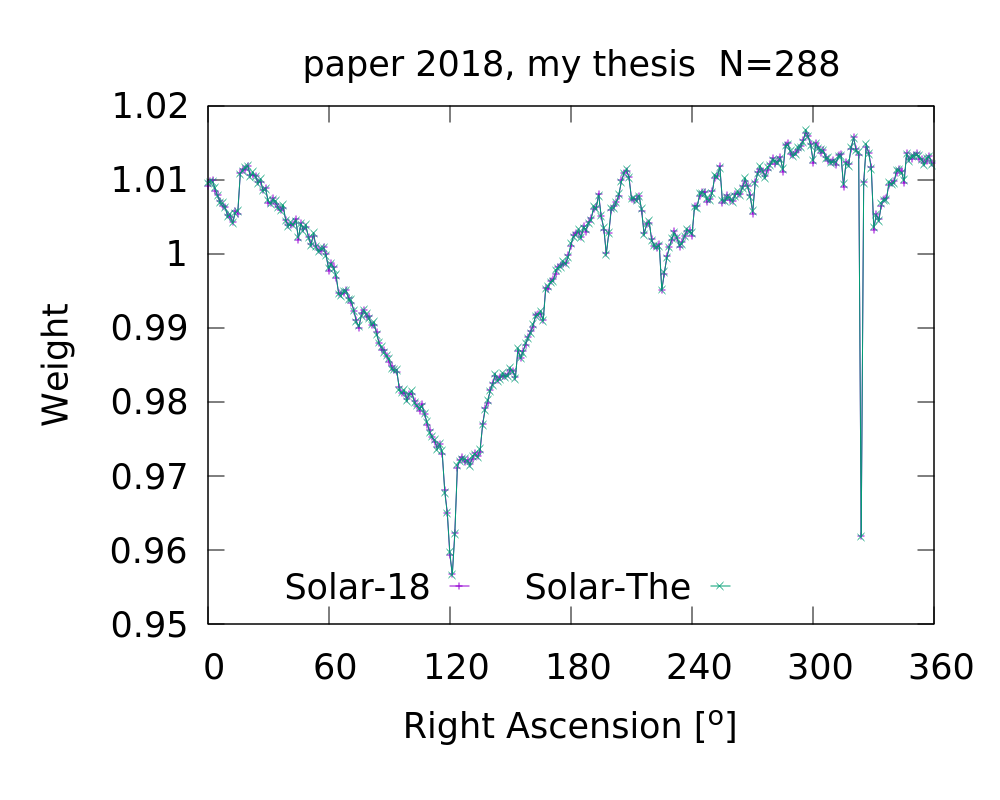
\includegraphics[width=0.45\textwidth]{Graficos/solar_my_and_paper_2018_in_288.png}
	\caption{Pesos para la frecuencia solar.}
	\label{fig:solar_288}
\end{figure}


\begin{figure}[H]
	\centering
	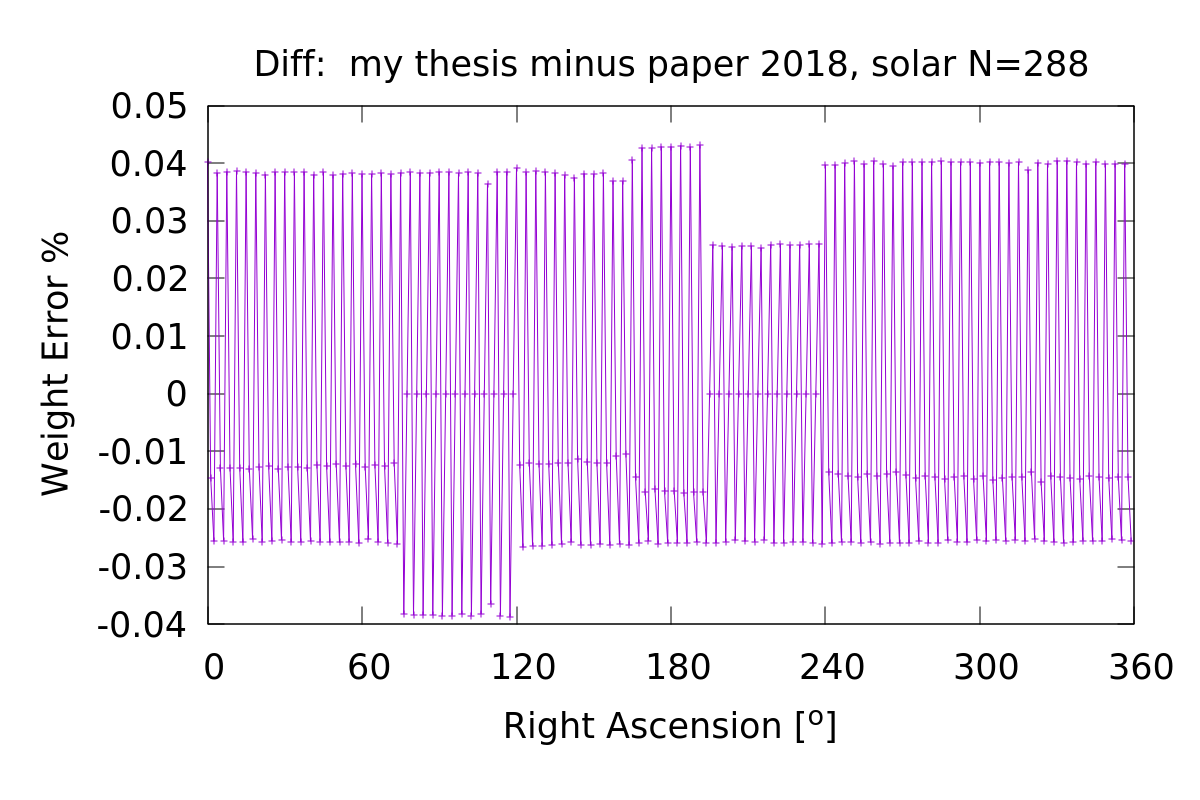
\includegraphics[width=0.45\textwidth]{Graficos/solar_my_and_paper_in_288_error.png}
	\caption{Error porcentual de los pesos de la frecuencia solar con respecto al paper 2018.}
	\label{fig:error_288_solar}
\end{figure}

Para la frecuencia anti-sidérea no hay mucha diferencia a los obtenido para el caso de N=360. Los pesos se muestran en la Fig.\,\ref{fig:anti_288} y el error con respecto al valor del paper se muestra en la Fig.\,\ref{fig:error_288_anti}.

\begin{figure}[H]
	\centering
	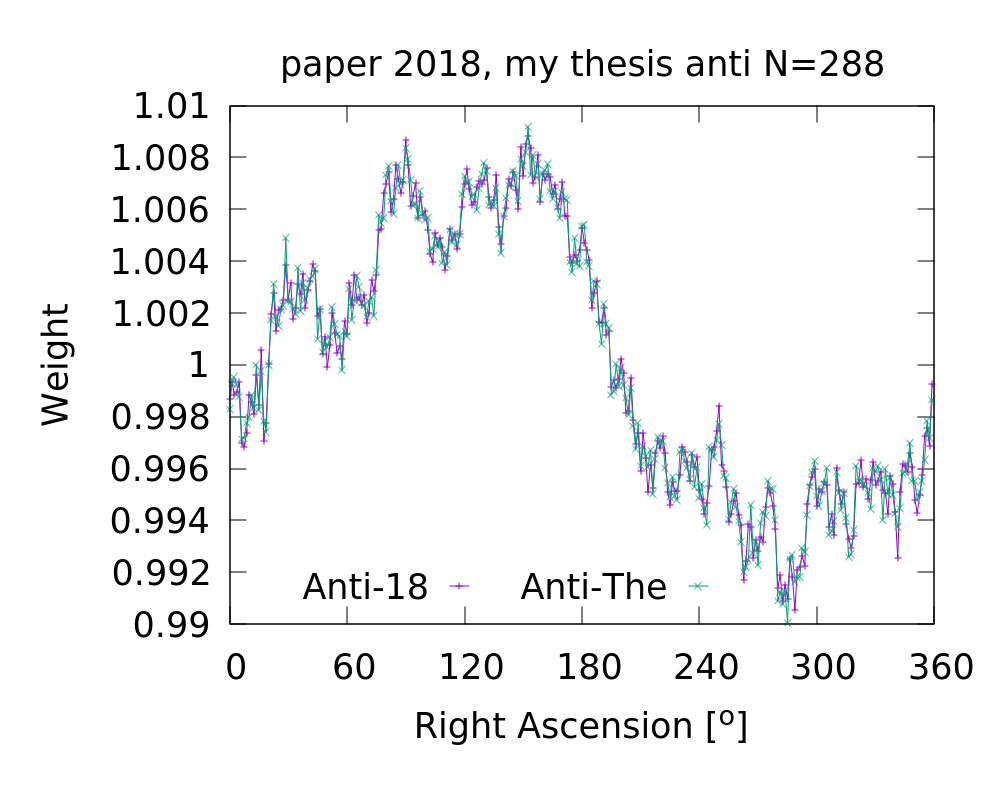
\includegraphics[width=0.45\textwidth]{Graficos/anti_my_and_paper_2018_in_288.png}
	\caption{Pesos para la frecuencia anti-sidérea}
	\label{fig:anti_288}
\end{figure}


\begin{figure}[H]
	\centering
	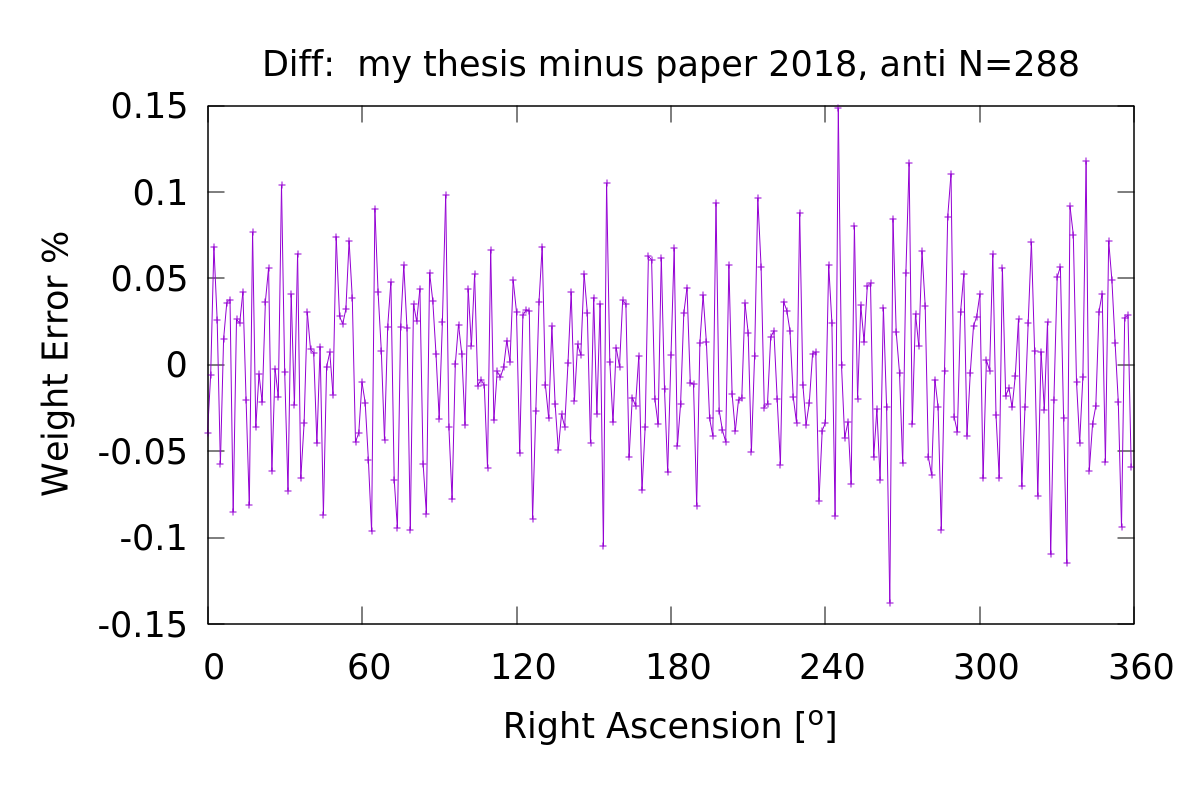
\includegraphics[width=0.45\textwidth]{Graficos/anti_my_and_paper_in_288_error.png}
	\caption{Error porcentual de los pesos de la frecuencia anti-sidérea con respecto al paper 2018.}
	\label{fig:error_288_anti}
\end{figure}



\end{document}
